\documentclass[11pt]{article}

% ---------- Packages ----------
\usepackage[margin=1in]{geometry}
\usepackage{amsmath, amssymb}
\usepackage{graphicx}
\usepackage{fancyhdr}
\usepackage{float}
\usepackage{listings}
\usepackage{xcolor}

\lstset{
    language=Matlab,
    basicstyle=\ttfamily\small,
    breaklines=true,
    breakatwhitespace=false,
    columns=fullflexible,
    showstringspaces=false,
    tabsize=4
}

% ---------- Paragraph Formatting ----------
\setlength{\parindent}{2pt}
\setlength{\parskip}{0.5em}

% ---------- Header ----------
\pagestyle{fancy}
\fancyhf{}
\lhead{ASEN 5090 Introduction to GNSS}
\rhead{Justin Le}
\cfoot{\thepage}

% ---------- Document ----------
\begin{document}

% ---------- Title ----------
\begin{center}
    {\Large \textbf{Homework 3}}\\[0.5em]
    {\large ASEN 5090 Introduction to GNSS}\\[0.5em]
    Justin Le\\
    \today
\end{center}

\vspace{1em}

\section*{Problem 1: GPS Observations}
\subsection*{(a.)}
\begin{lstlisting}[language=Matlab]
% Read rinex file

rinexData = rinexread('NIST00USA_R_20262310000_01D_30S_MO.rnx');

GPS_rinexData = rinexData.GPS;

PRN_number = 5;
PRN_index = GPS_rinexData.SatelliteID == PRN_number;
PRN05_GPS_rinexData = GPS_rinexData(PRN_index,:);

[NIST_GPS_week, NIST_GPS_TOW] = utc2gpstime(PRN05_GPS_rinexData.Time);
ephem_time_s = NIST_GPS_week.*604800 + NIST_GPS_TOW;

% Nan gap the discontinuous 
gap_idx = [false; diff(ephem_time_s) > 1.5*median(diff(ephem_time_s))];
PRN05_GPS_rinexData.C1C(gap_idx) = NaN;
PRN05_GPS_rinexData.S1C(gap_idx) = NaN;
PRN05_GPS_rinexData.C1W(gap_idx) = NaN;
PRN05_GPS_rinexData.D1C(gap_idx) = NaN;
\end{lstlisting}
\subsection*{(b.)}
\begin{figure}[H]
    \centering
    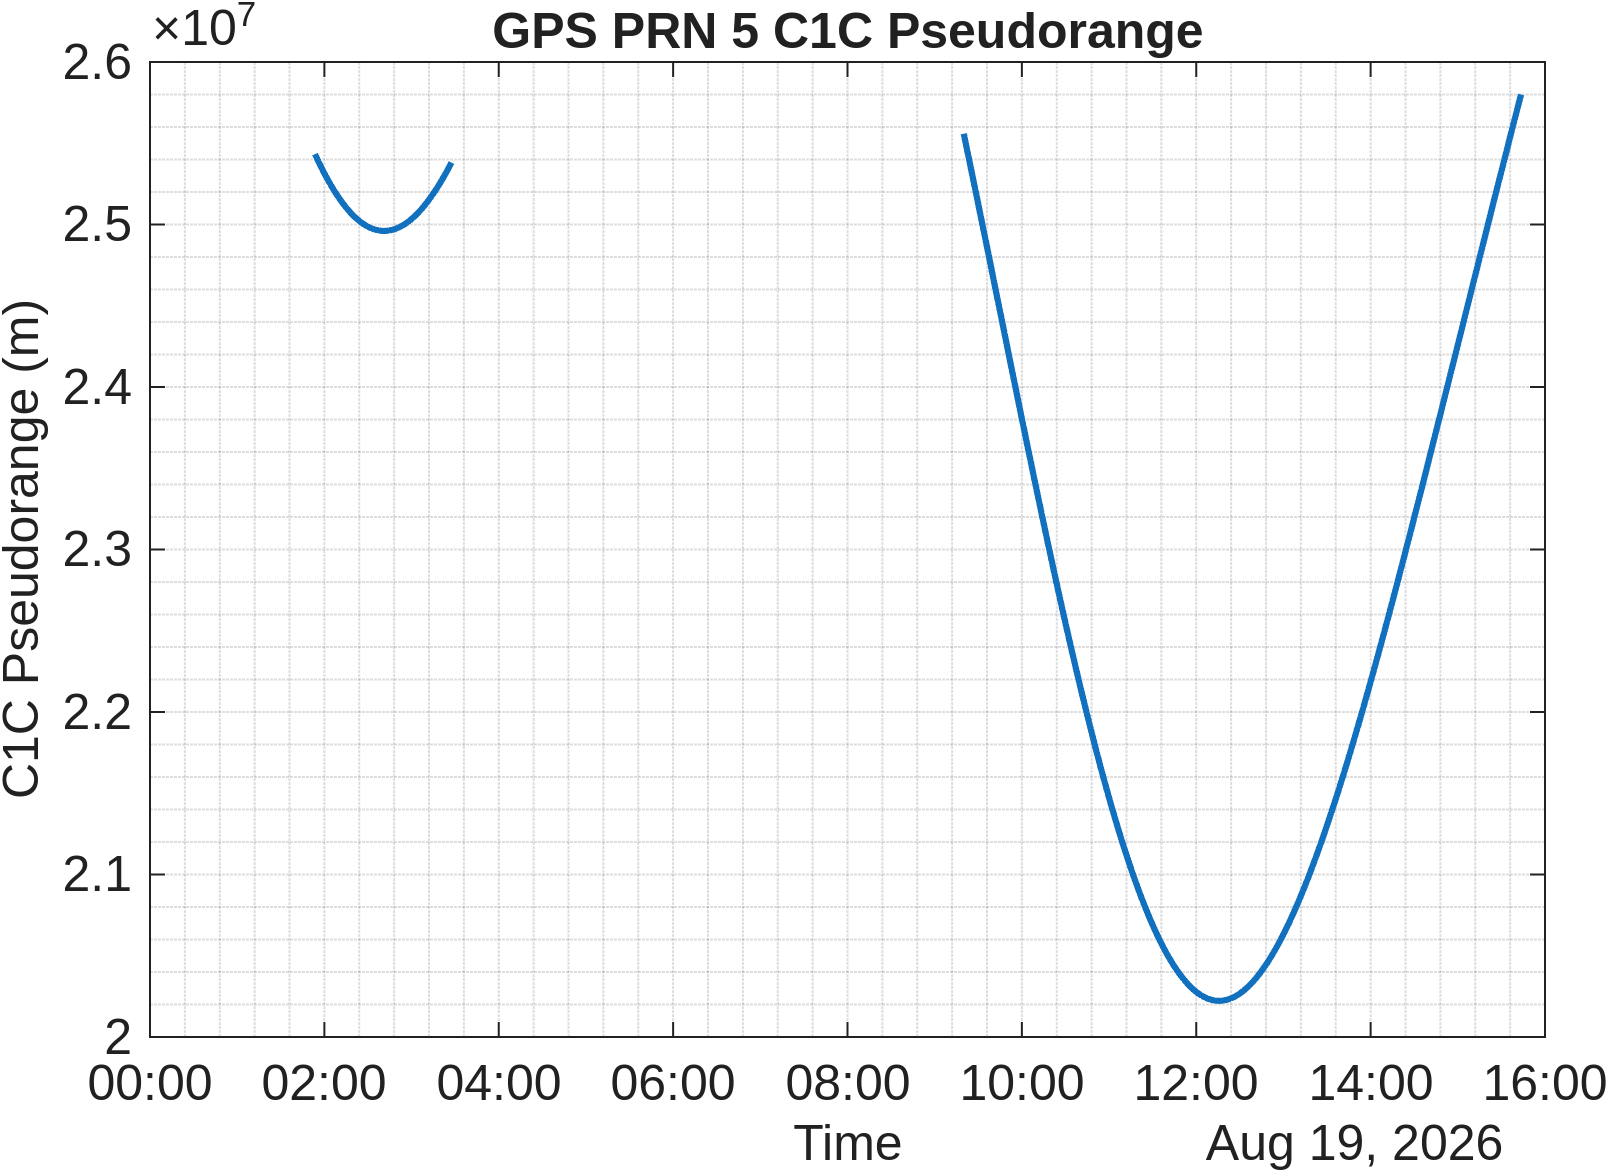
\includegraphics[width=0.6\textwidth]{../MATLAB/figures/HW3_P1_C1C_PRN5.png}
    \caption{C1C Pseudorange for PRN5}
    \label{fig:C1C Pseudorange for PRN5}
\end{figure}

\subsection*{(c.)}
\begin{figure}[H]
    \centering
    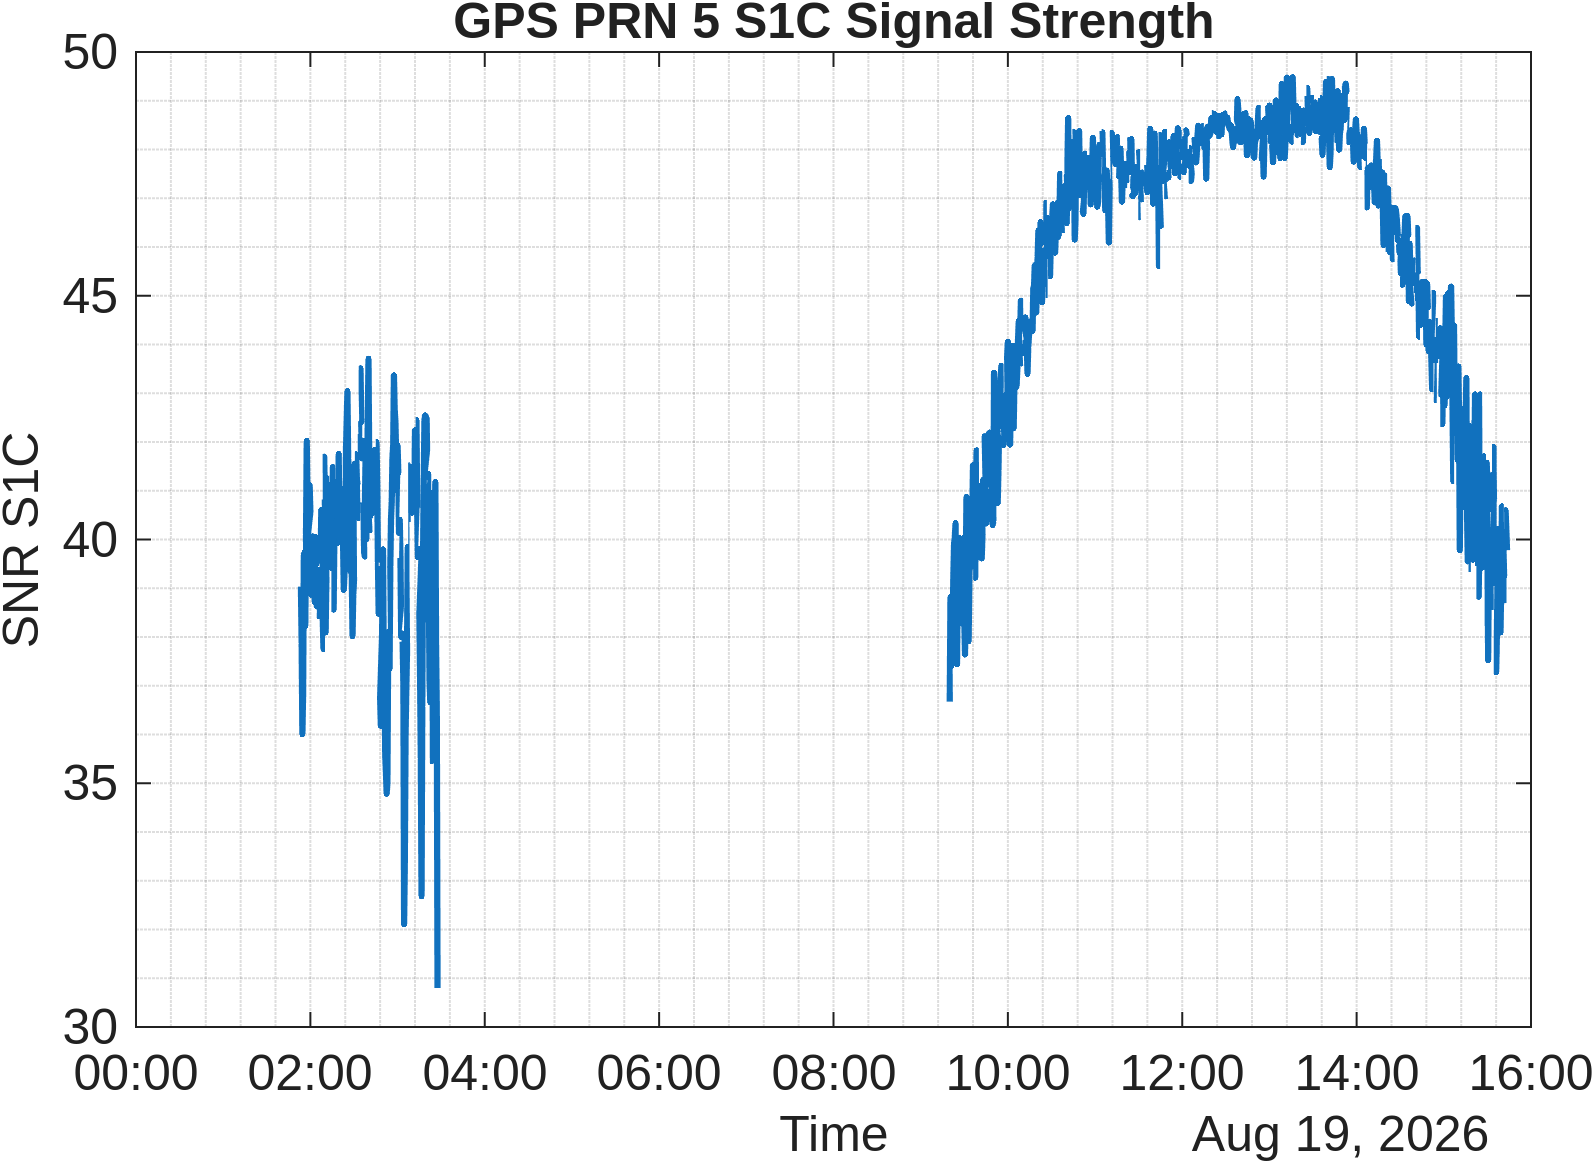
\includegraphics[width=0.6\textwidth]{../MATLAB/figures/HW3_P1_S1C_PRN5.png}
    \caption{S1C SNR for PRN5}
    \label{fig:S1C SNR for PRN5}
\end{figure}

\subsection*{(d.)}
\begin{figure}[H]
    \centering
    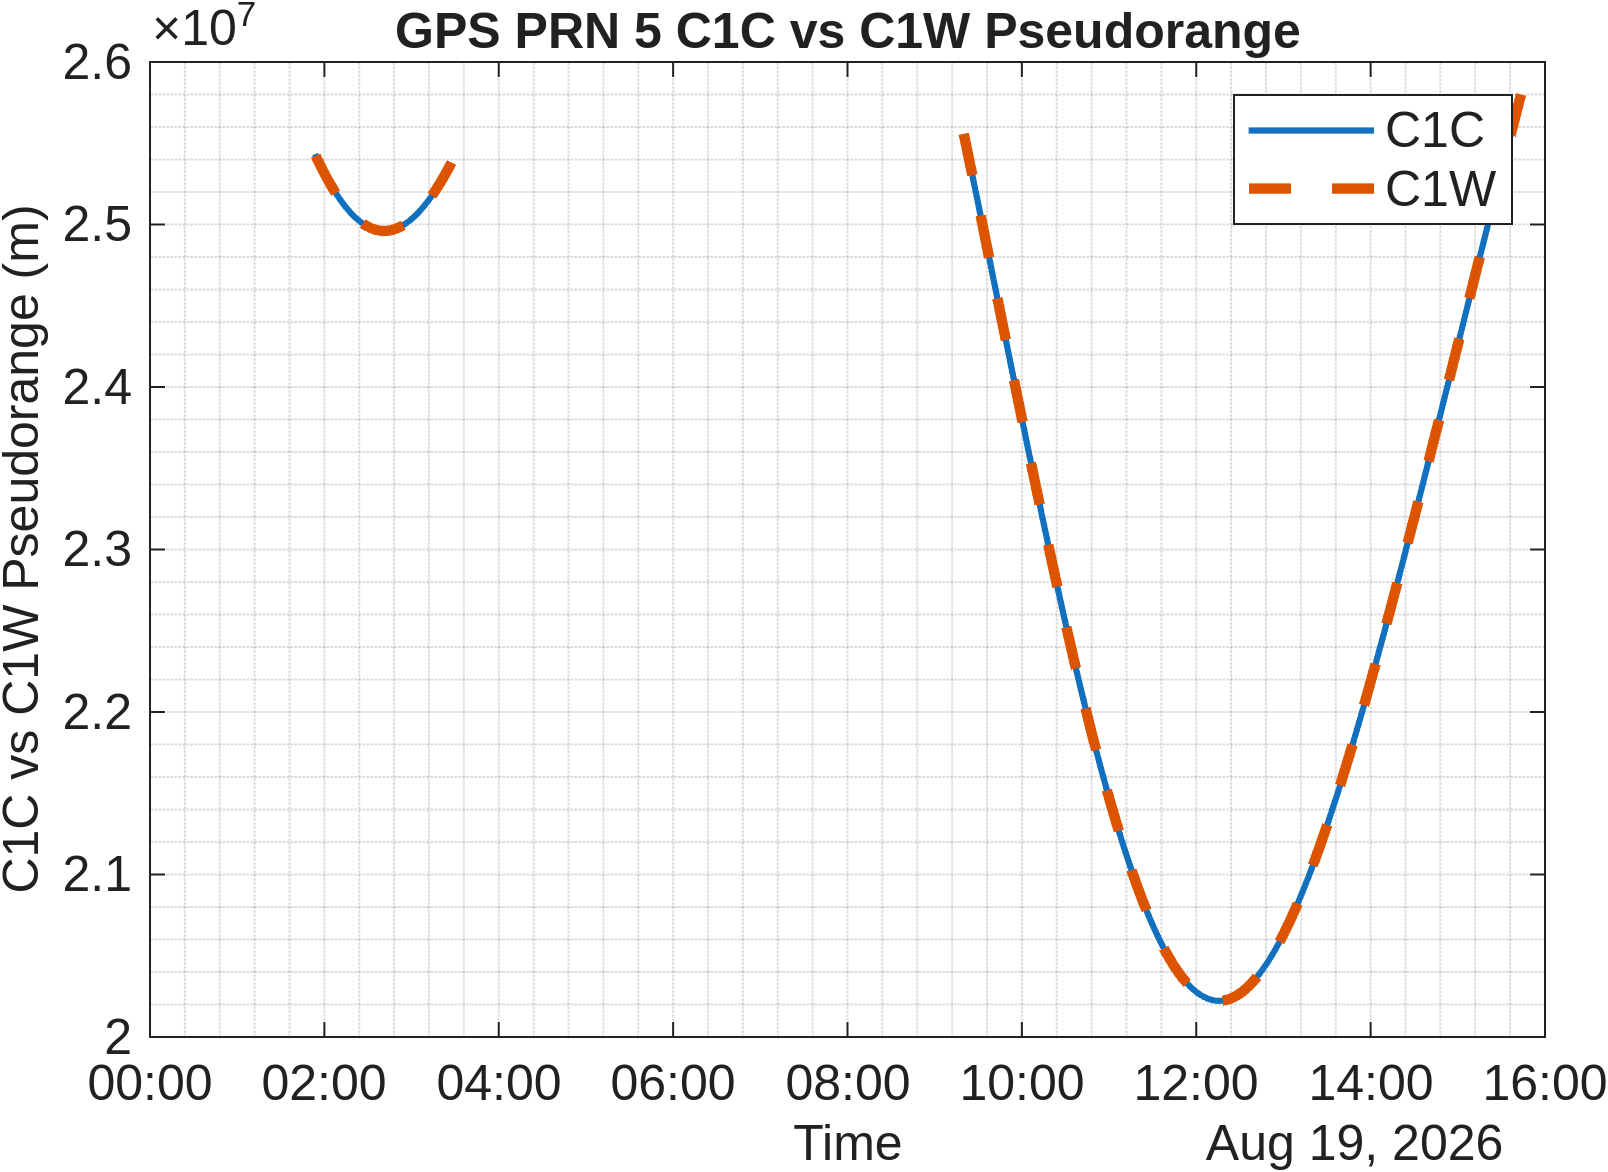
\includegraphics[width=0.6\textwidth]{../MATLAB/figures/HW3_P1_C1C_C1W_PRN5.png}
    \caption{C1C and C1W Pseudorange for PRN5}
    \label{fig:C1C and C1W Pseudorange for PRN5PRN5}
\end{figure}

TODO: describe the differences yada yada


\section*{Problem 2: GPS Positions Based on Ephemeris Data}
\subsection*{(a.)}
\begin{lstlisting}[language=Matlab]
% Use read clean to read in ephermides
clean_GPSbroadcast = read_clean_GPSbroadcast('brdc2310.26n', true);

% Read in sp3 ephem like HW2 
sp3 = read_sp3('IGS0OPSFIN_20262310000_01D_15M_ORB.SP3');
satPRN = extract_sp3_prn(sp3);

[health,satPos,satVel,satClkCorr] = eph2pvt2025(clean_GPSbroadcast, [satPRN(5).week_number satPRN(5).TOW_s], 5);

\end{lstlisting}
\subsection*{(b.)}
\begin{figure}[H]
    \centering
    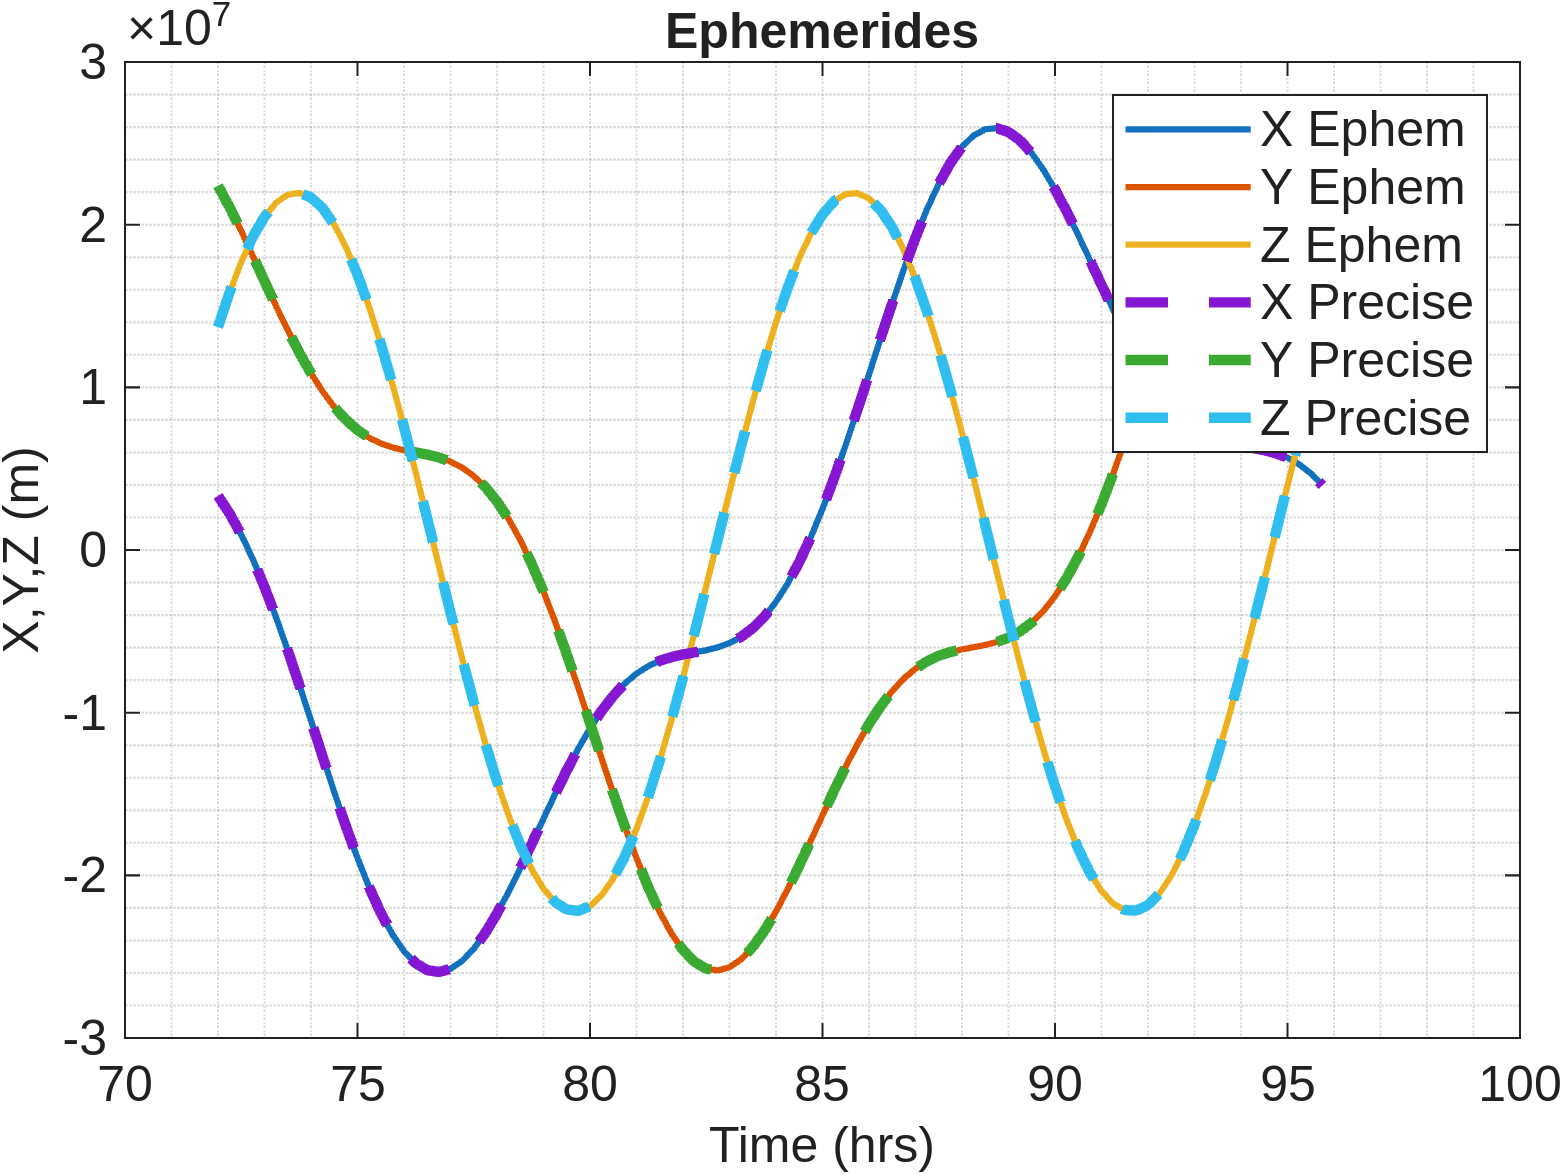
\includegraphics[width=0.6\textwidth]{../MATLAB/figures/HW3_P2_ephem_precise_PRN5.png}
    \caption{Ephemeris vs Precise}
    \label{fig:Ephemeris vs Precise}
\end{figure}

\begin{figure}[H]
    \centering
    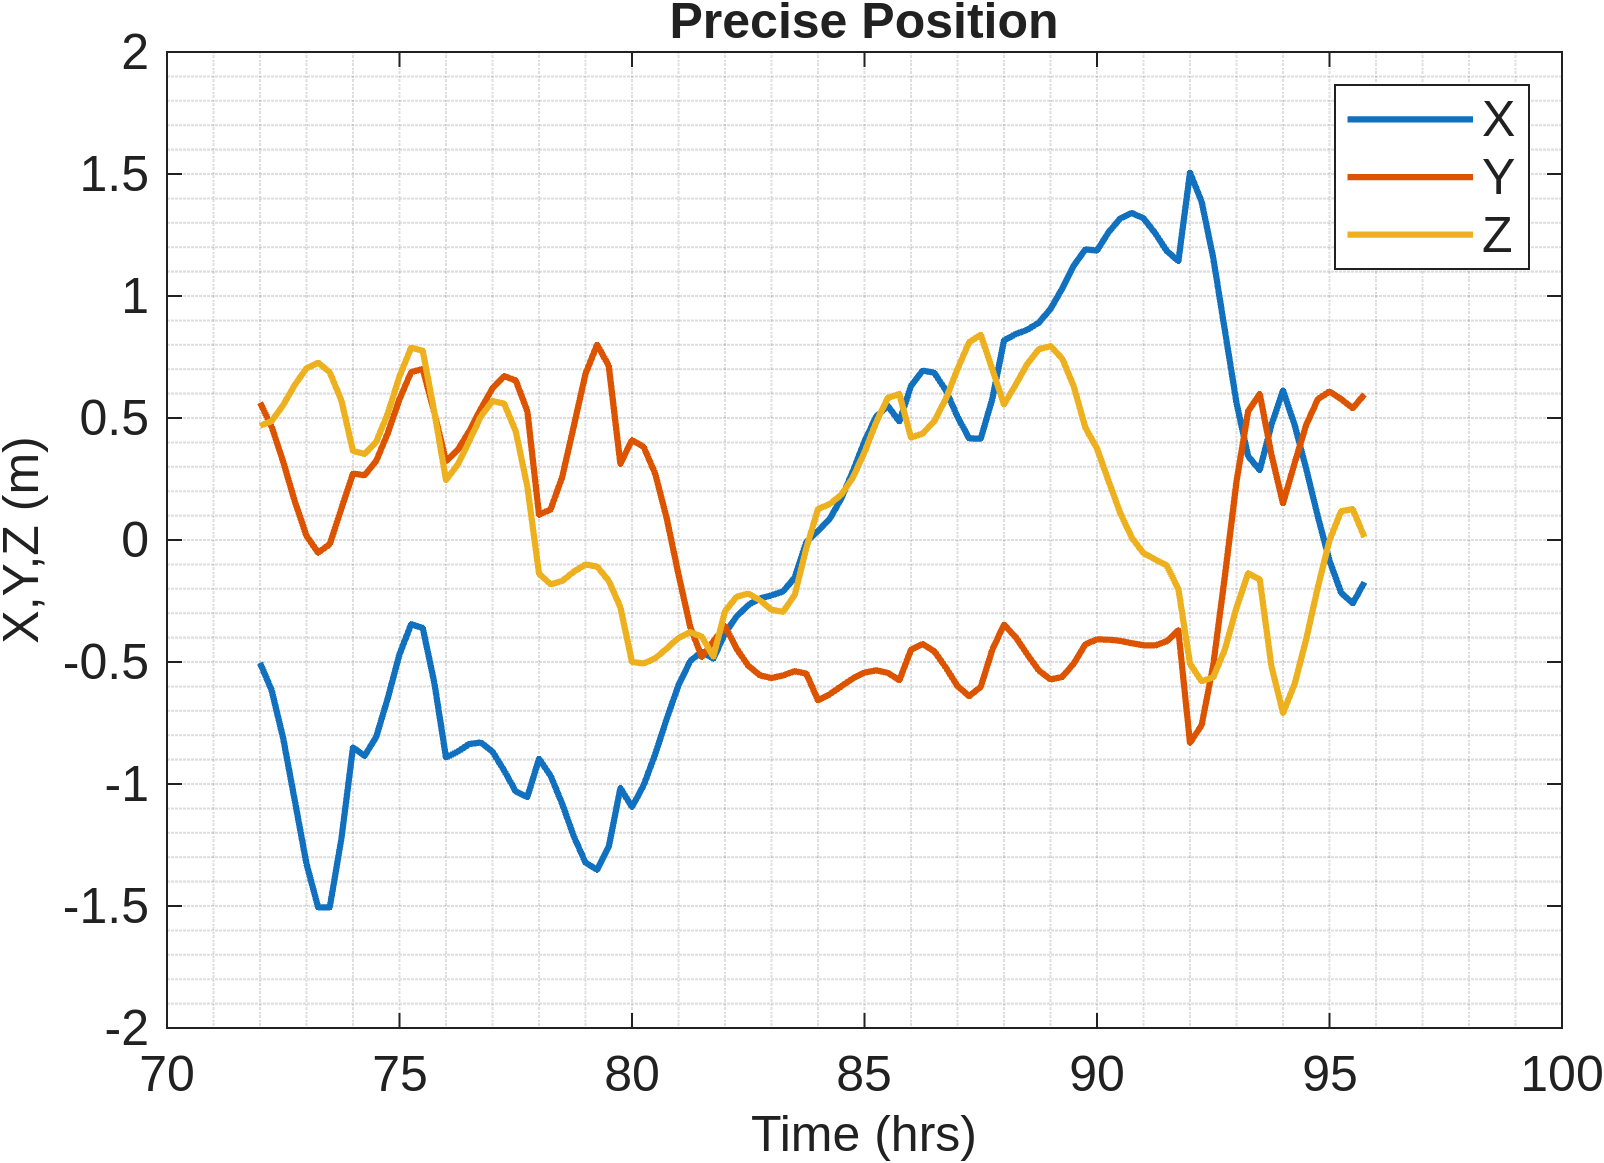
\includegraphics[width=0.6\textwidth]{../MATLAB/figures/HW3_P2_xyz_residual_PRN5.png}
    \caption{Ephemeris vs Precise}
    \label{fig:Ephemeris vs Precise Residuals}
\end{figure}

TODO: Comment on differences
\subsection*{(c.)}
\begin{figure}[H]
    \centering
    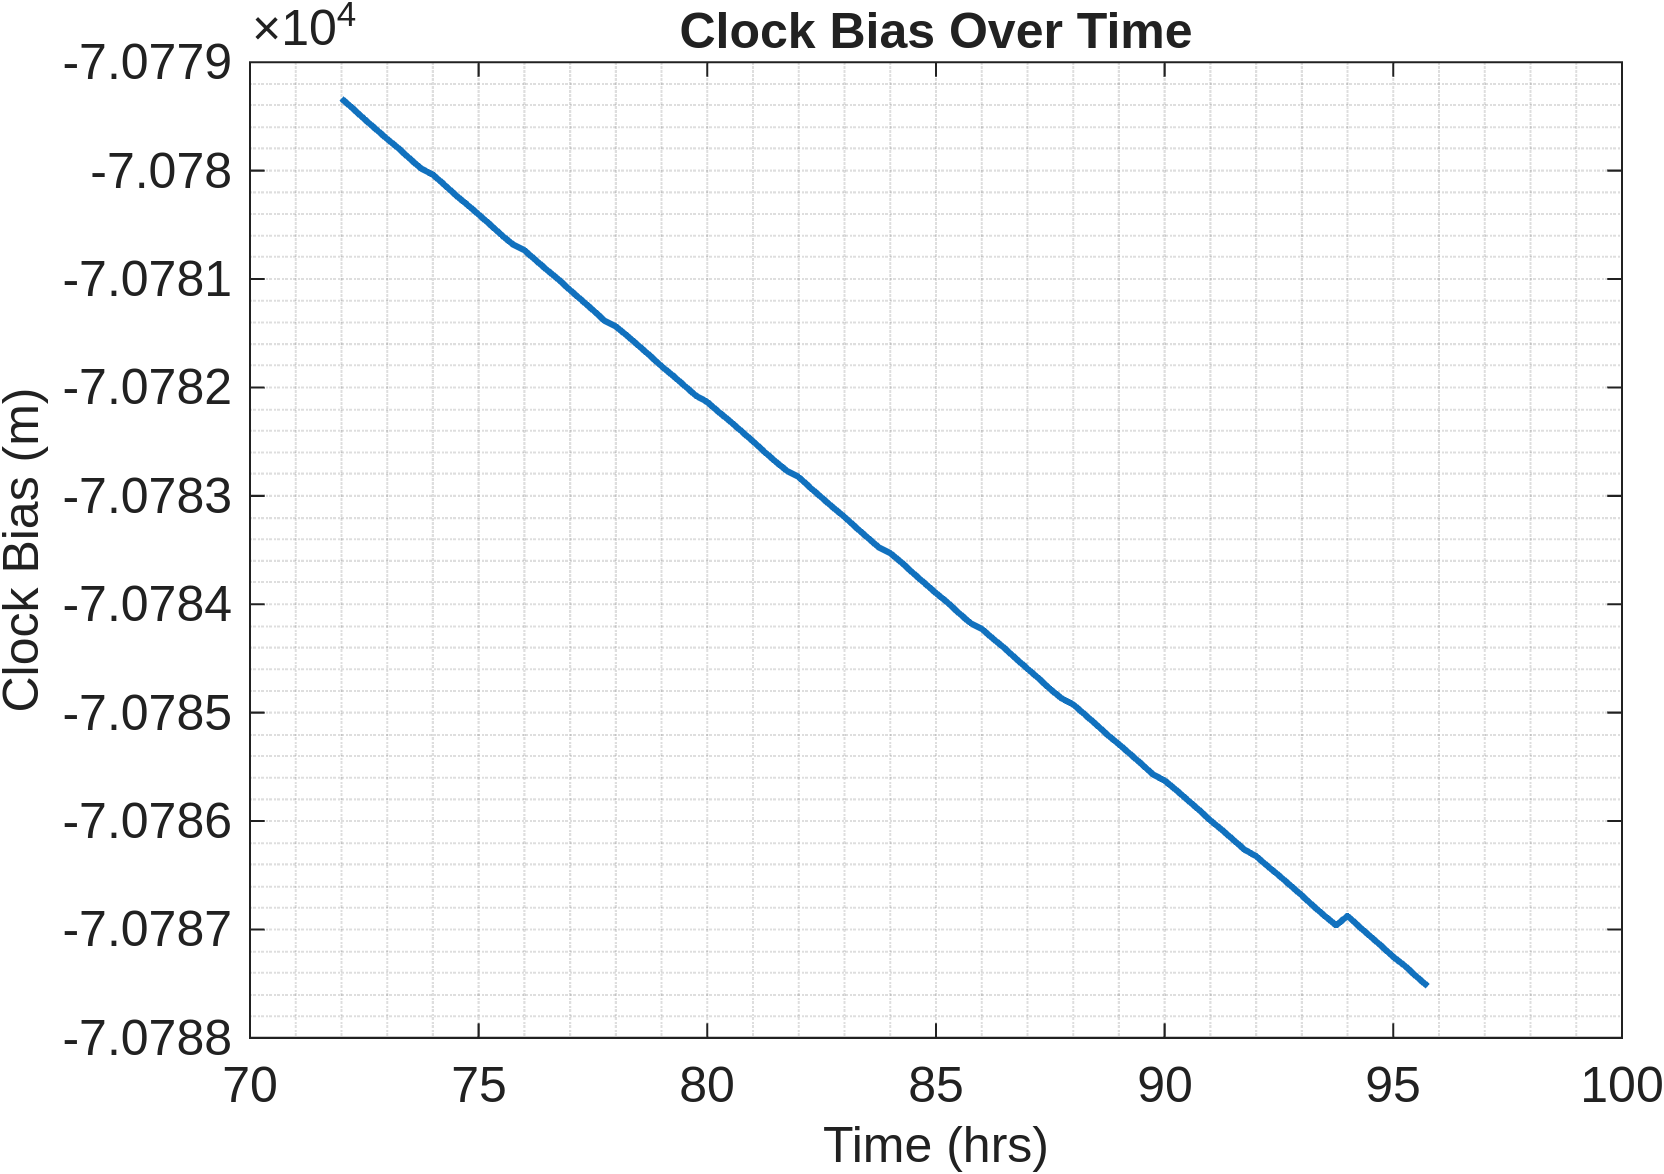
\includegraphics[width=0.6\textwidth]{../MATLAB/figures/HW3_P2_clock_bias_PRN5.png}
    \caption{Clock Bias}
    \label{fig:Clock Bias}
\end{figure}

\section*{Problem 3: GPS Expected Range}
\subsection*{(a.)}
\begin{figure}[H]
    \centering
    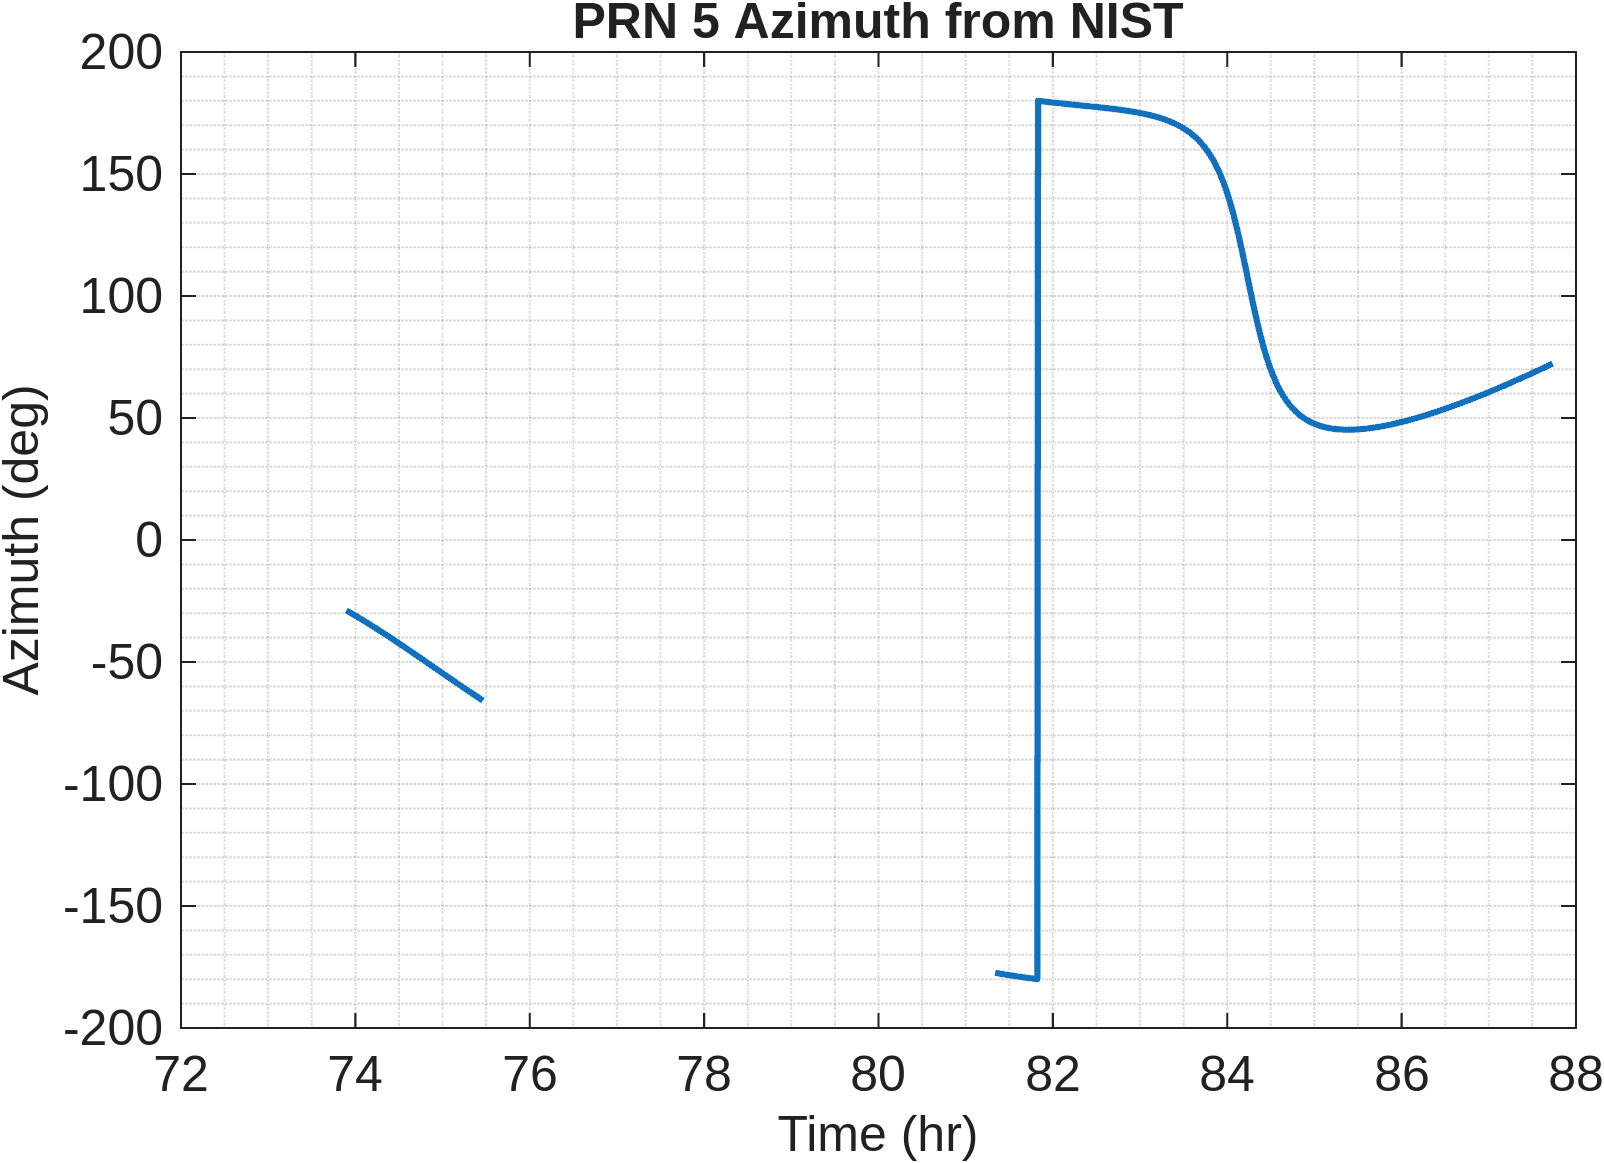
\includegraphics[width=0.6\textwidth]{../MATLAB/figures/HW3_P3_azimuth_PRN5.png}
    \caption{PRN5 Azimuth}
    \label{fig:PRN5 Azimuth}
\end{figure}

\begin{figure}[H]
    \centering
    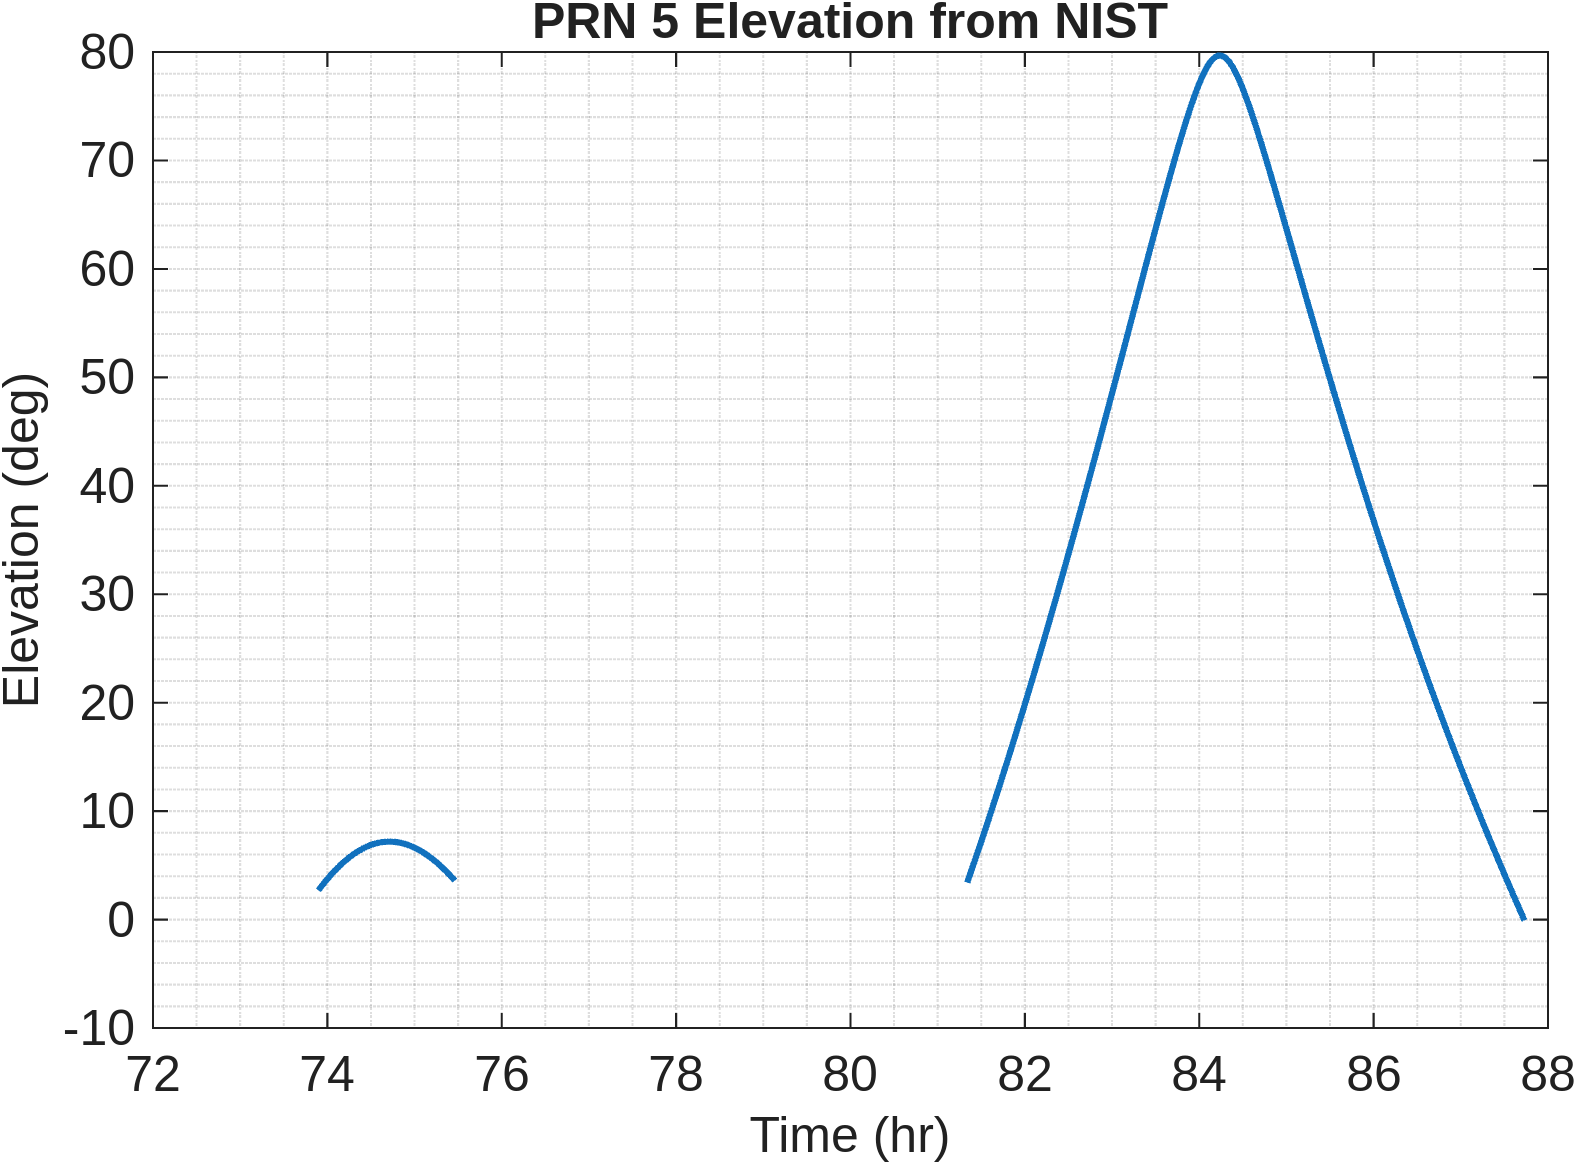
\includegraphics[width=0.6\textwidth]{../MATLAB/figures/HW3_P3_elevation_PRN5.png}
    \caption{PRN5 Elevation}
    \label{fig:PRN5 Elevation}
\end{figure}

\begin{figure}[H]
    \centering
    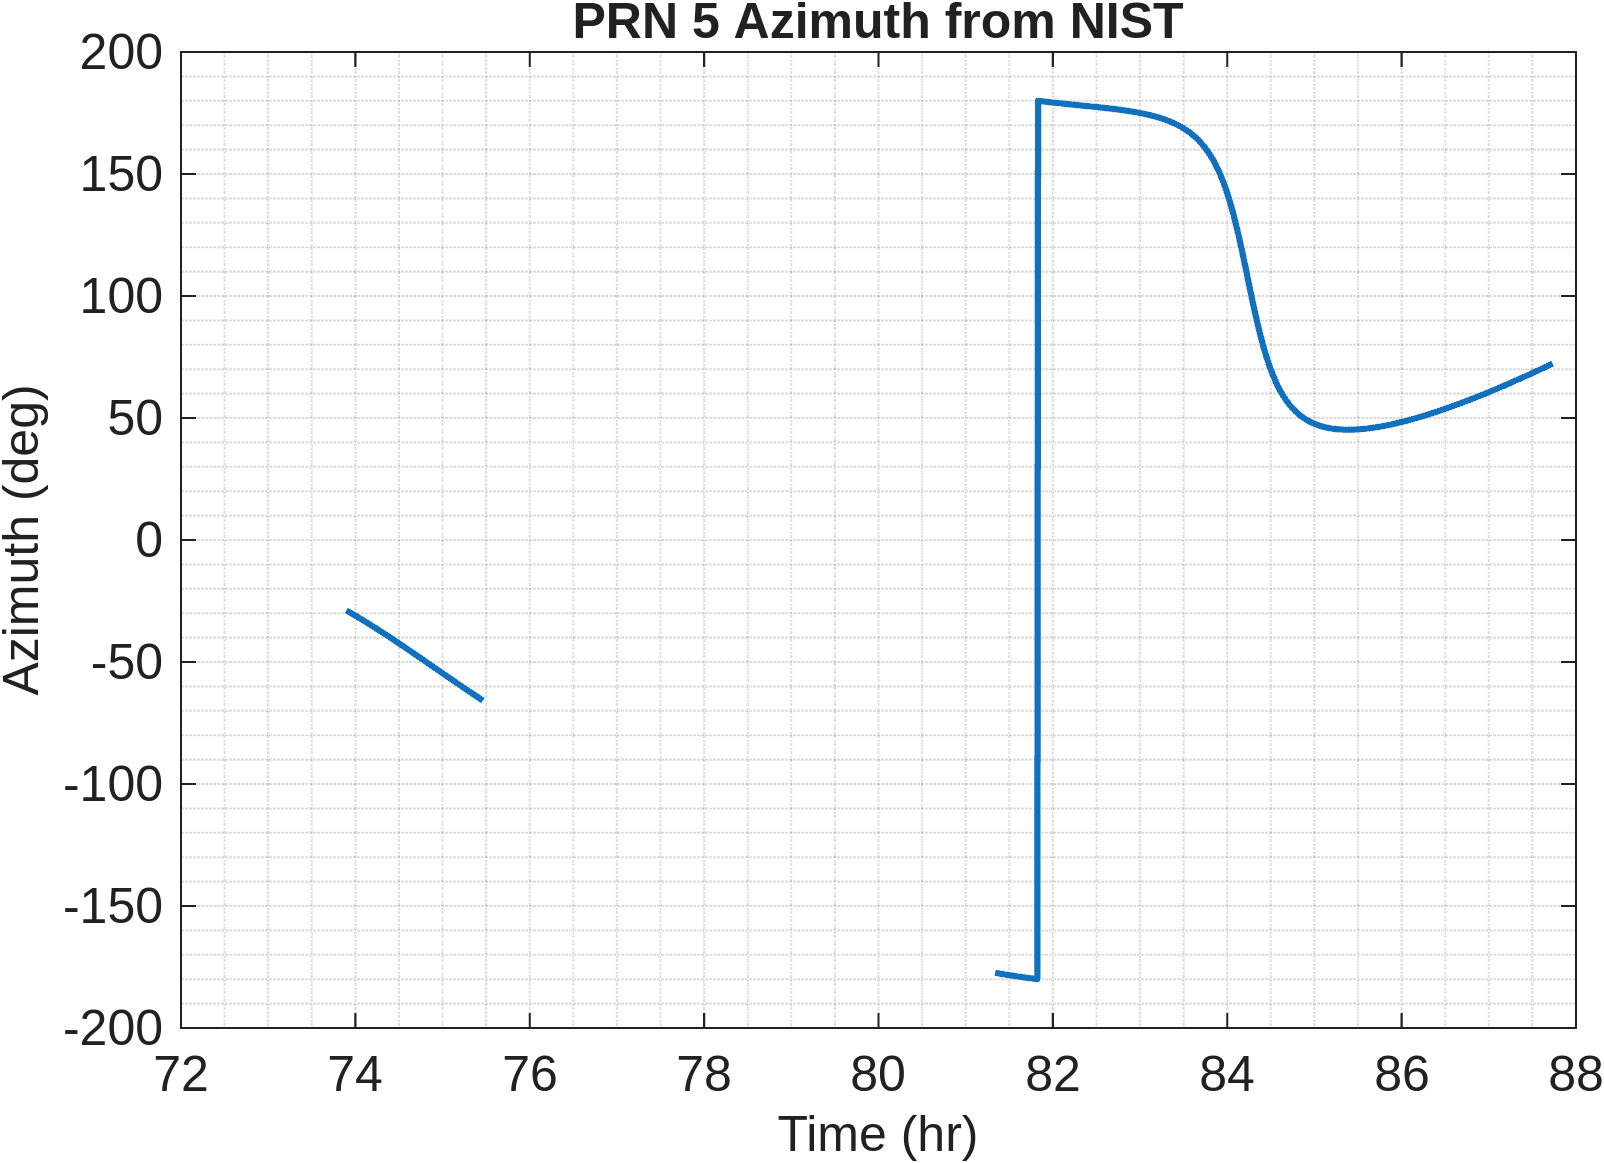
\includegraphics[width=0.6\textwidth]{../MATLAB/figures/HW3_P3_azimuth_PRN5.png}
    \caption{PRN5 Azimuth}
    \label{fig:PRN5 Azimuth}
\end{figure}

\begin{figure}[H]
    \centering
    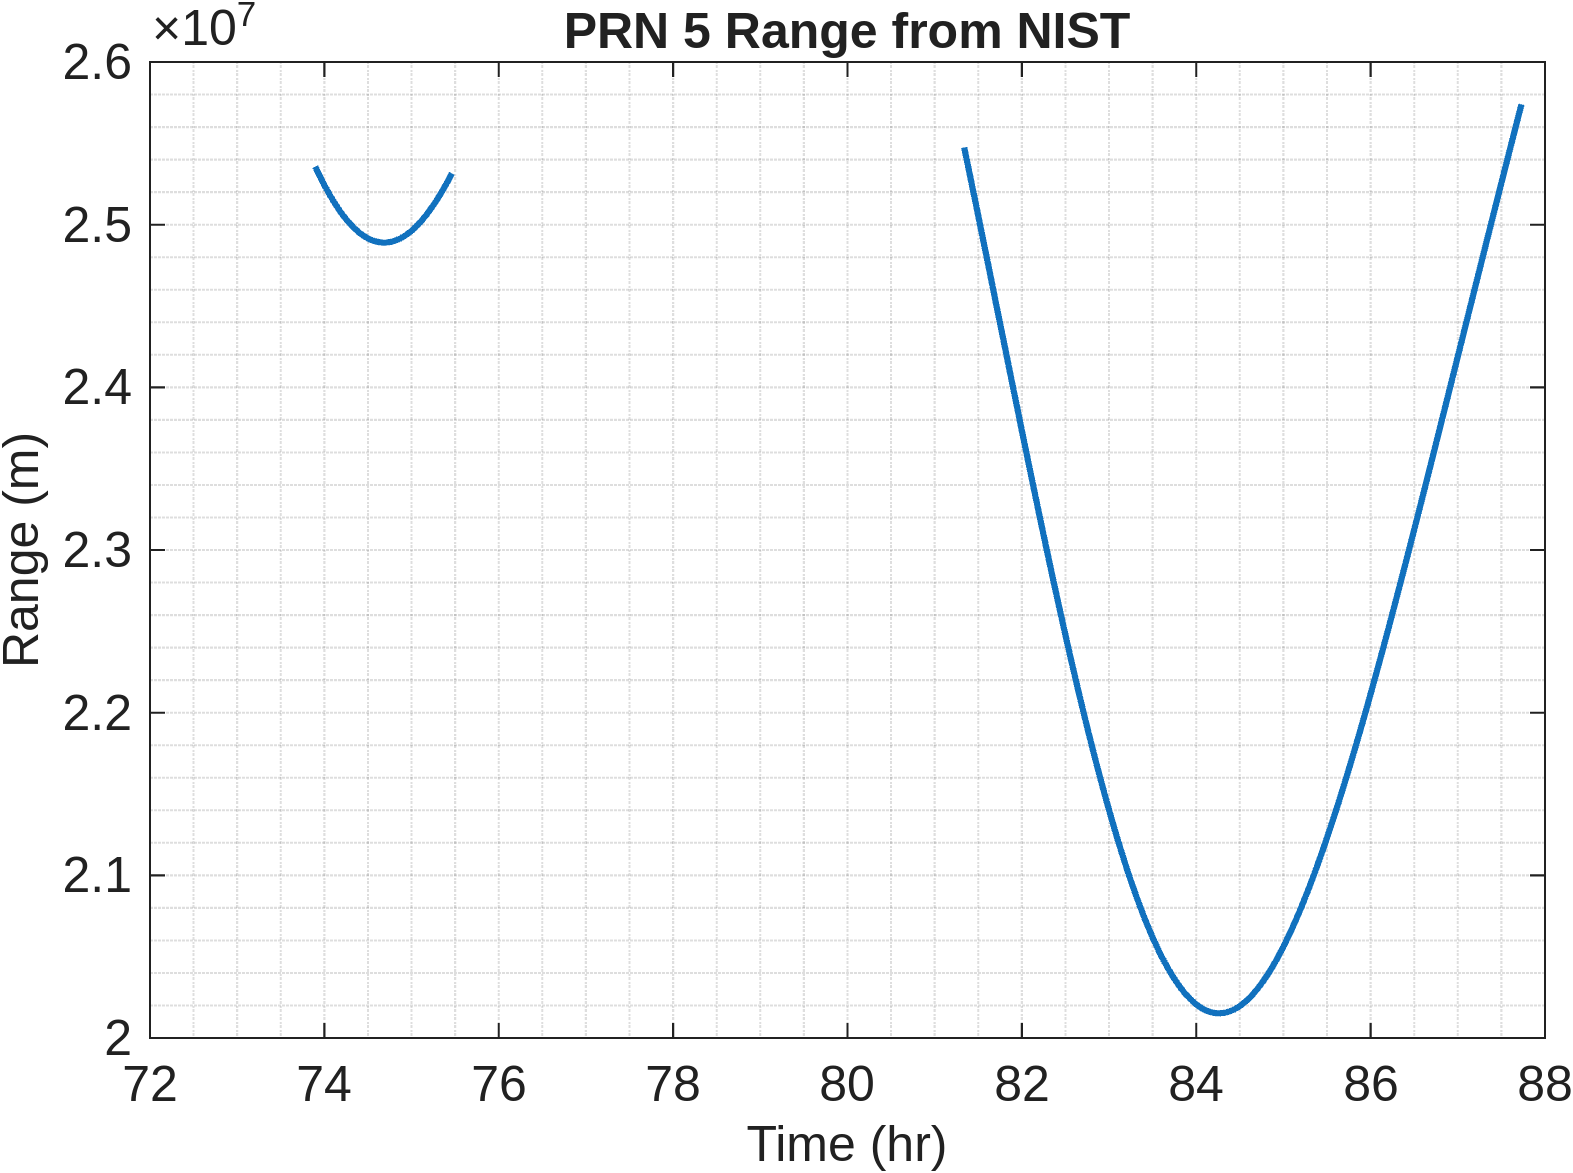
\includegraphics[width=0.6\textwidth]{../MATLAB/figures/HW3_P3_range_PRN5.png}
    \caption{PRN5 Range}
    \label{fig:PRN5 Range}
\end{figure}

\subsection*{(b.)}
\begin{figure}[H]
    \centering
    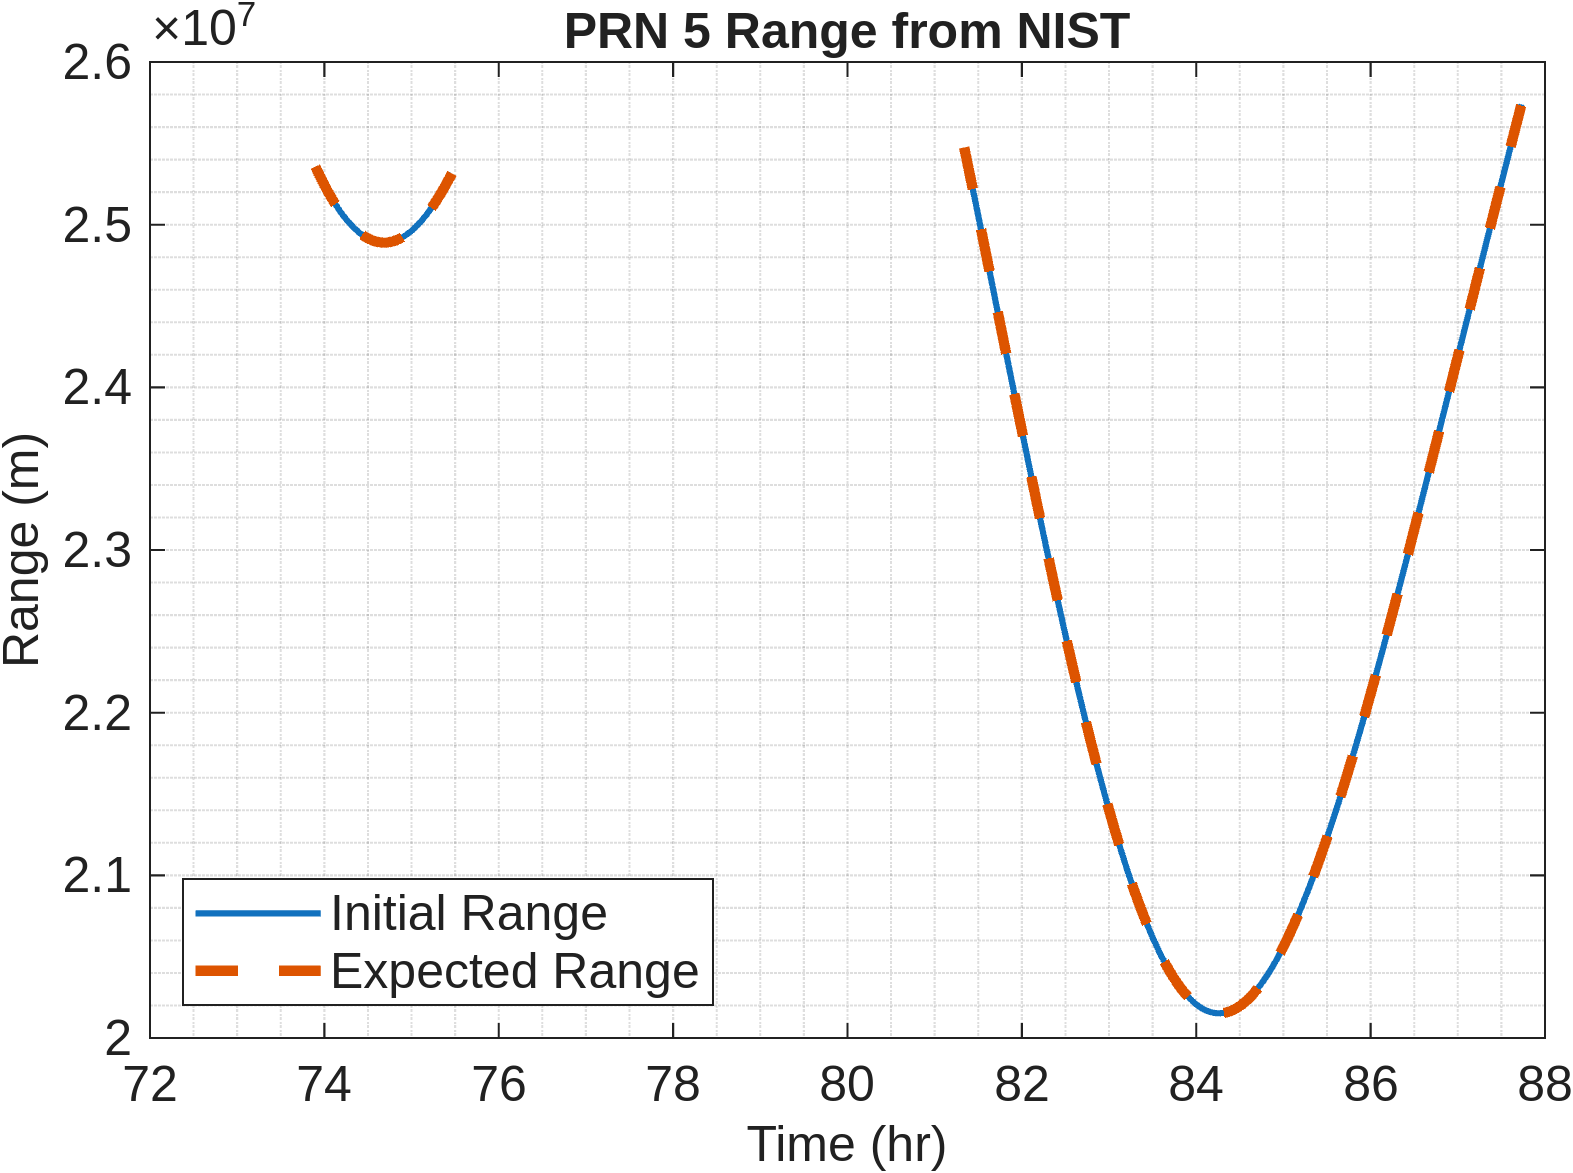
\includegraphics[width=0.6\textwidth]{../MATLAB/figures/HW3_P3_initial_range_vs_expected_PRN5.png}
    \caption{PRN5 Range Initial vs Expected}
    \label{fig:PRN5 Range Initial vs Expected}
\end{figure}

\begin{figure}[H]
    \centering
    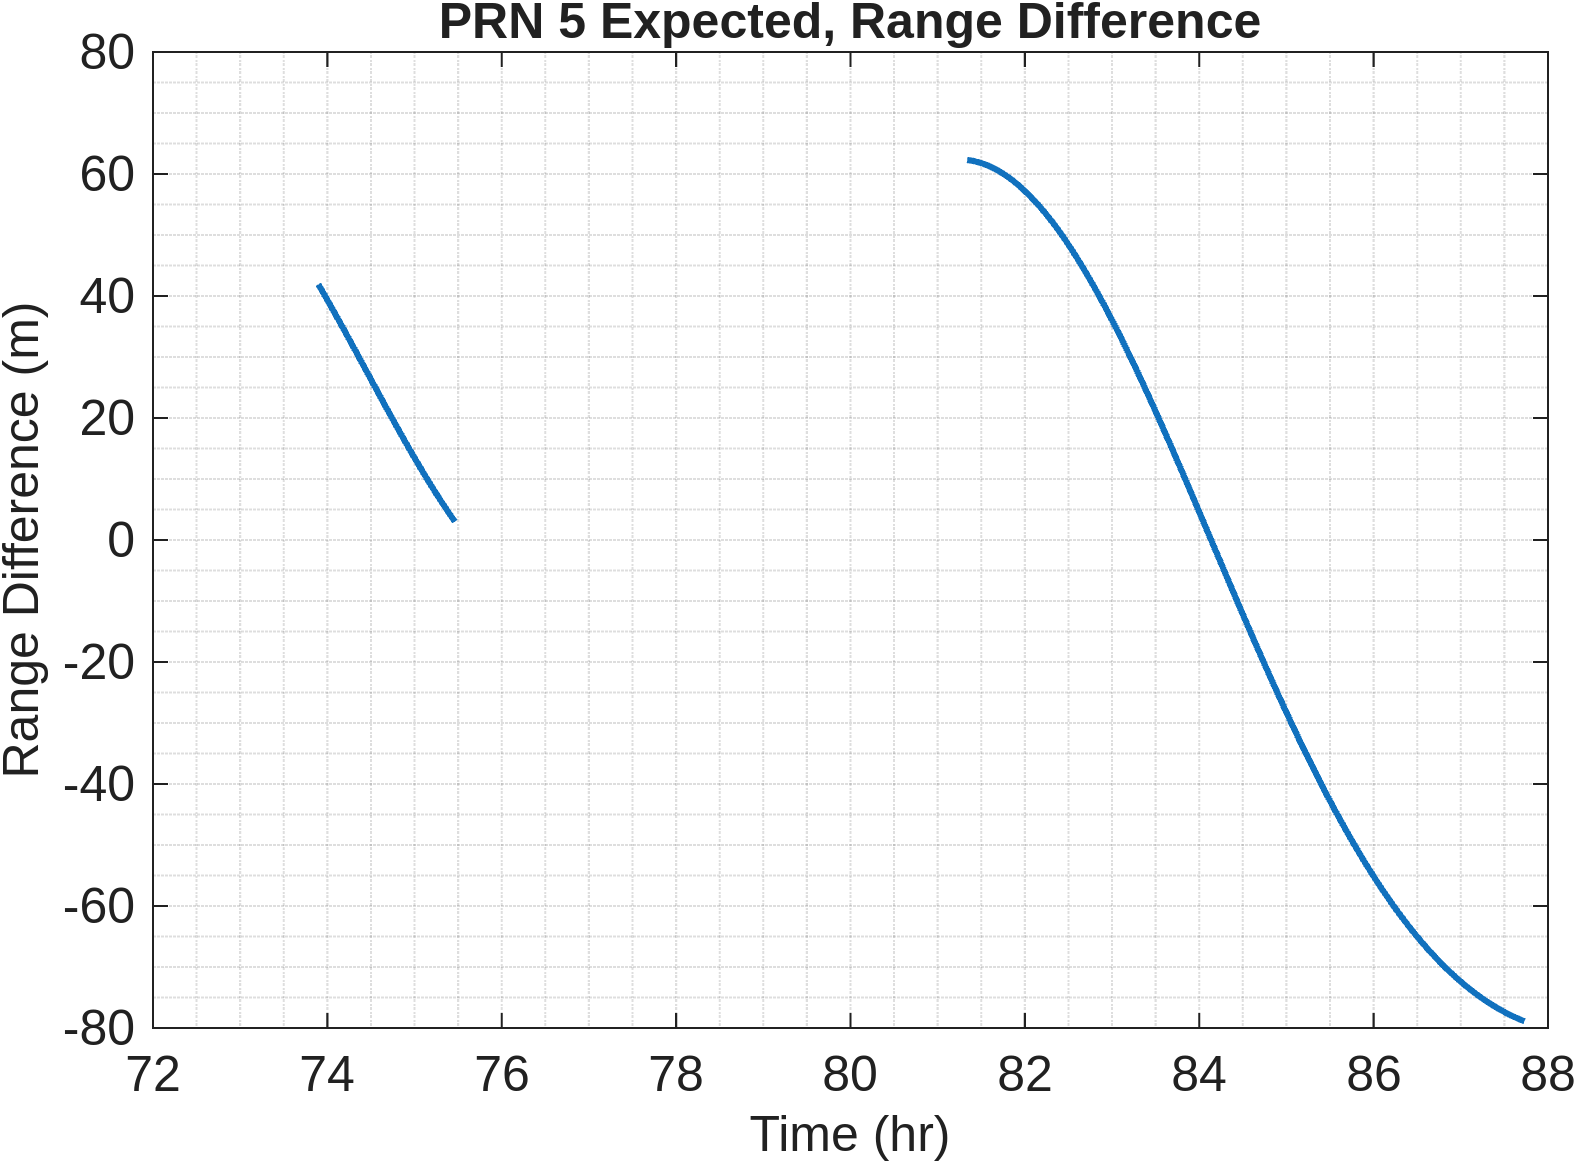
\includegraphics[width=0.6\textwidth]{../MATLAB/figures/HW3_P3_range_difference_PRN5.png}
    \caption{PRN5 Range Initial vs Expected Residual}
    \label{fig:PRN5 Range Initial vs Expected Residual}
\end{figure}
TODO: report largest difference found.

\section*{Problem 4: Observed Minus Computed (Expected) Range}
\begin{figure}[H]
    \centering
    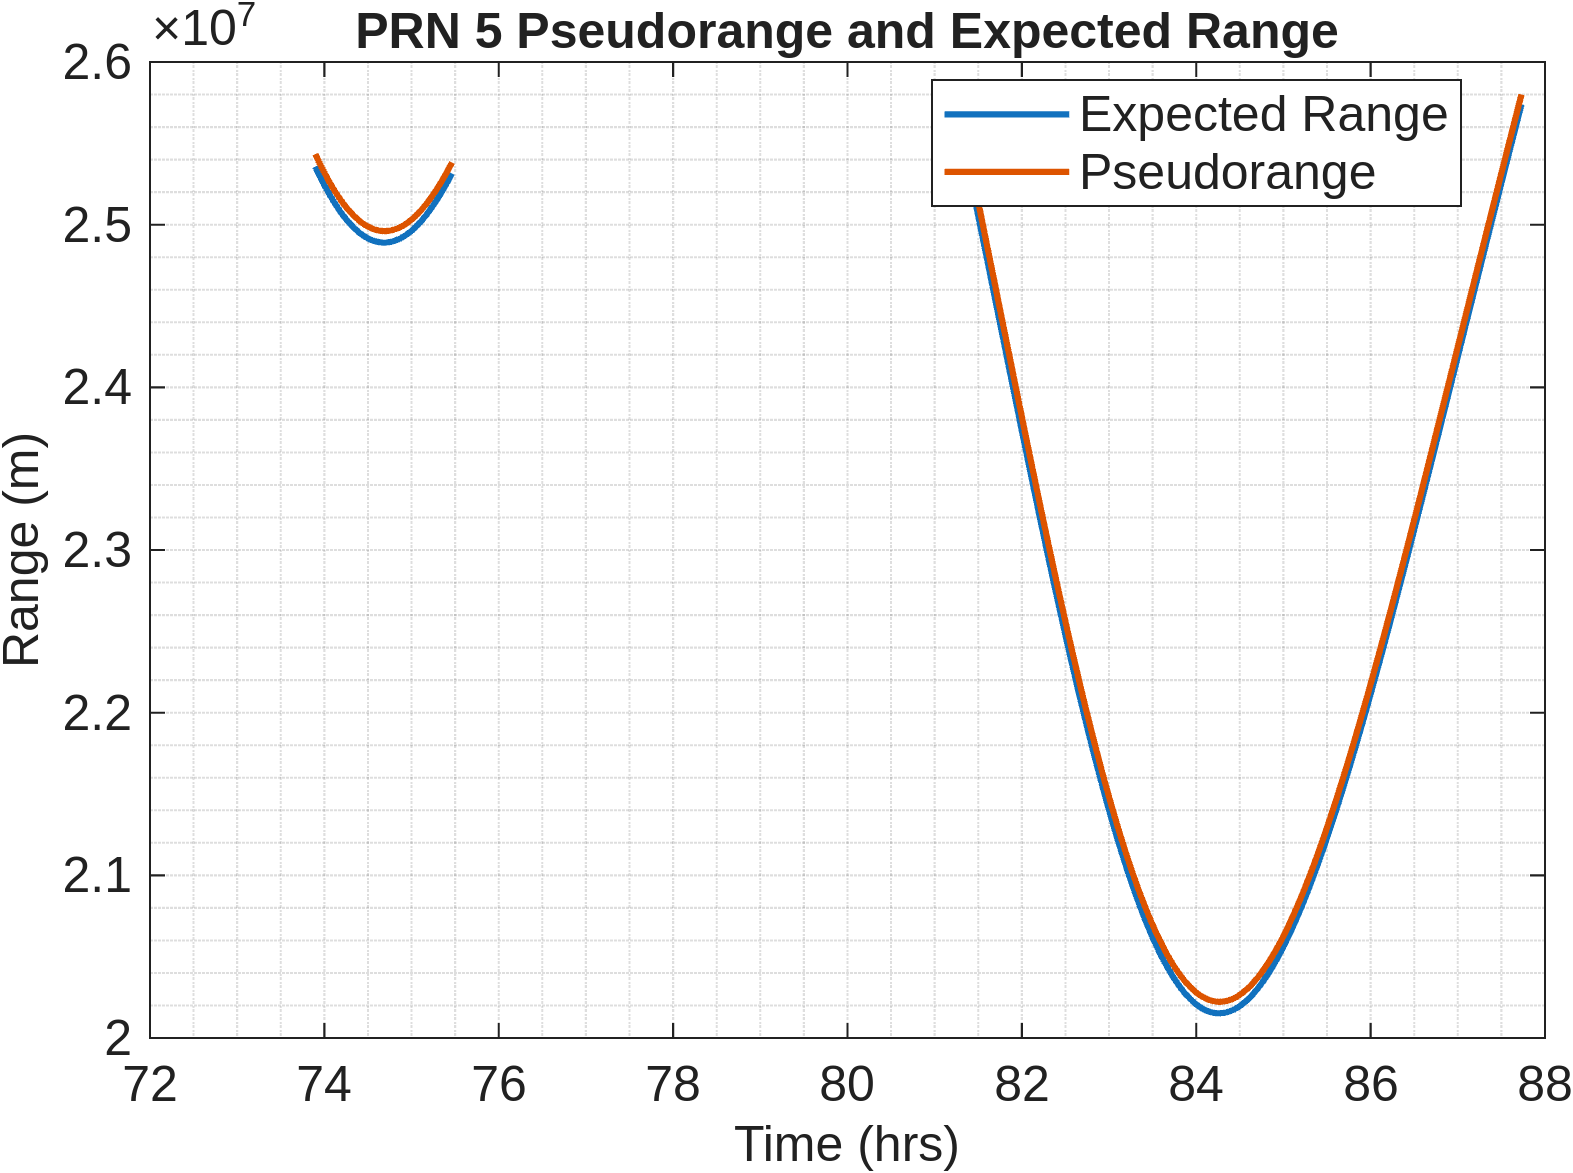
\includegraphics[width=0.6\textwidth]{../MATLAB/figures/HW3_P4_pseudorange_vs_expected_PRN5.png}
    \caption{PRN5 C1C Pseudorange vs Expected Range}
    \label{fig:PRN5 C1C Pseudorange vs Expected Range}
\end{figure}

\begin{figure}[H]
    \centering
    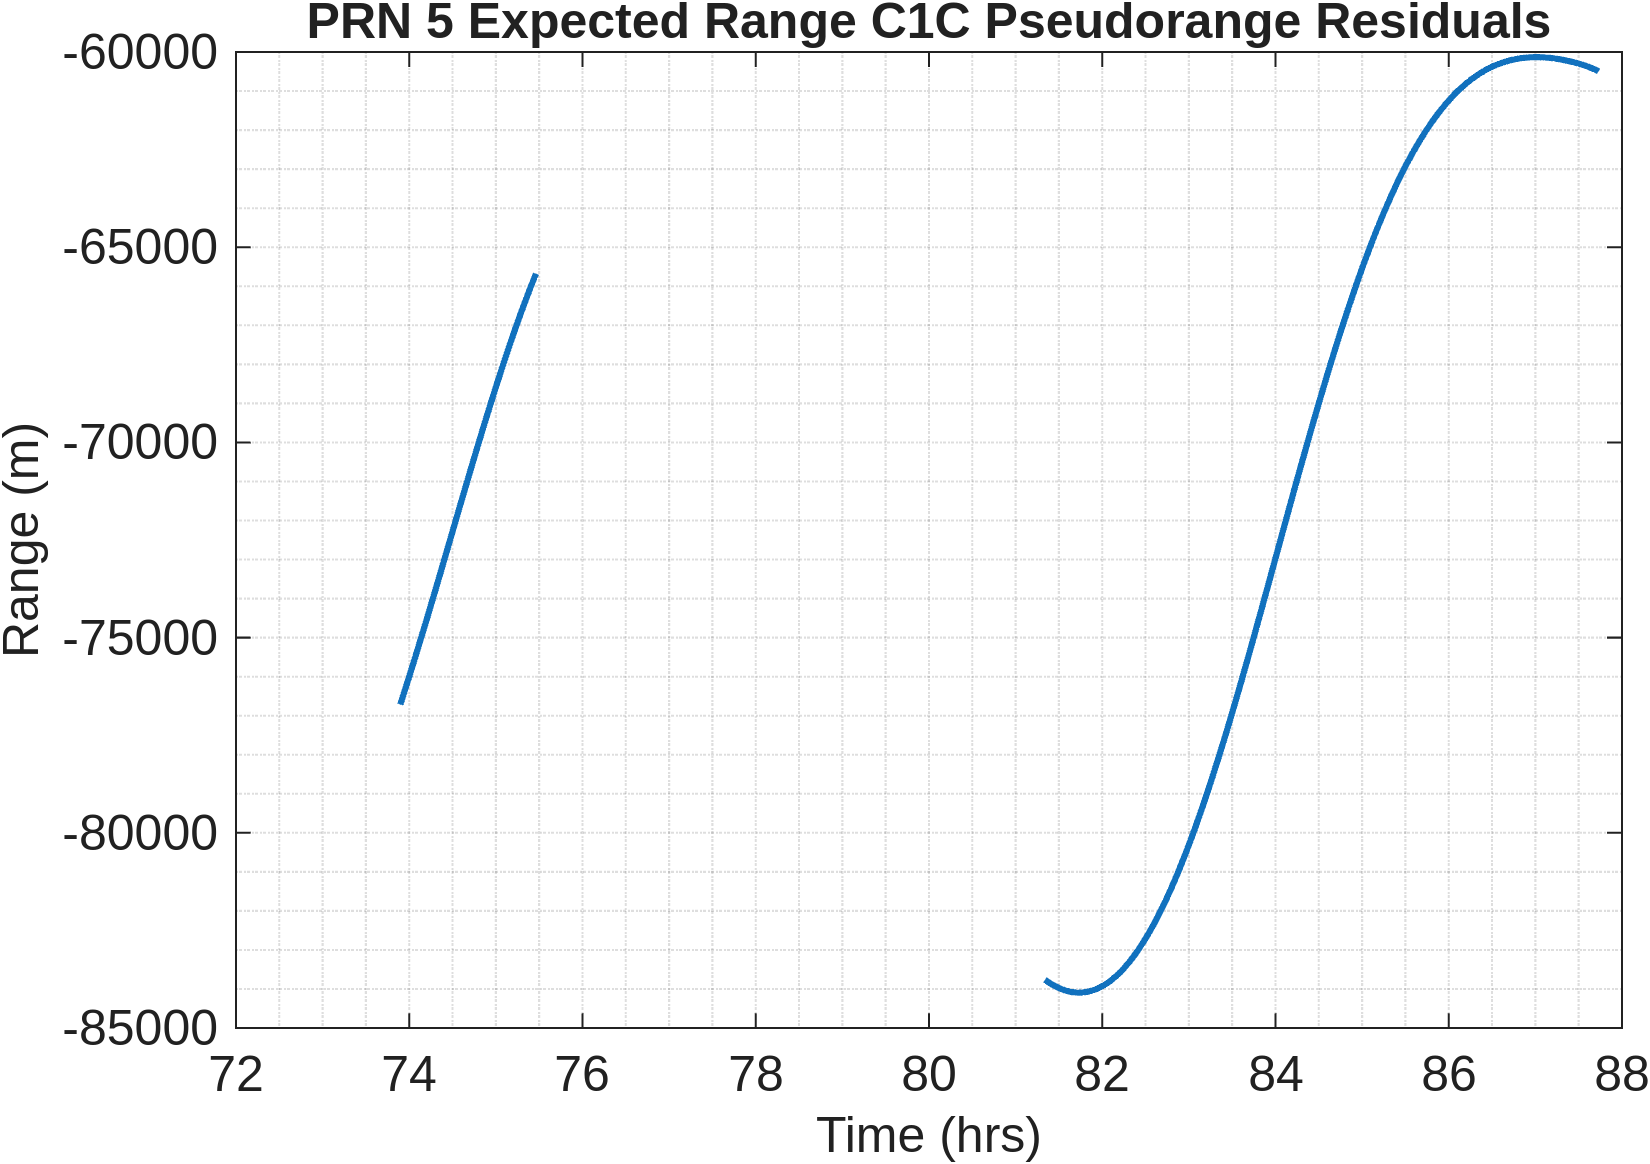
\includegraphics[width=0.6\textwidth]{../MATLAB/figures/HW3_P4_residuals_PRN5.png}
    \caption{PRN5 C1C Pseudorange vs Expected Range Residuals}
    \label{fig:PRN5 C1C Pseudorange vs Expected Range Residuals}
\end{figure}


\section*{Problem 5: Repeat for another PRN}

\begin{figure}[H]
    \centering
    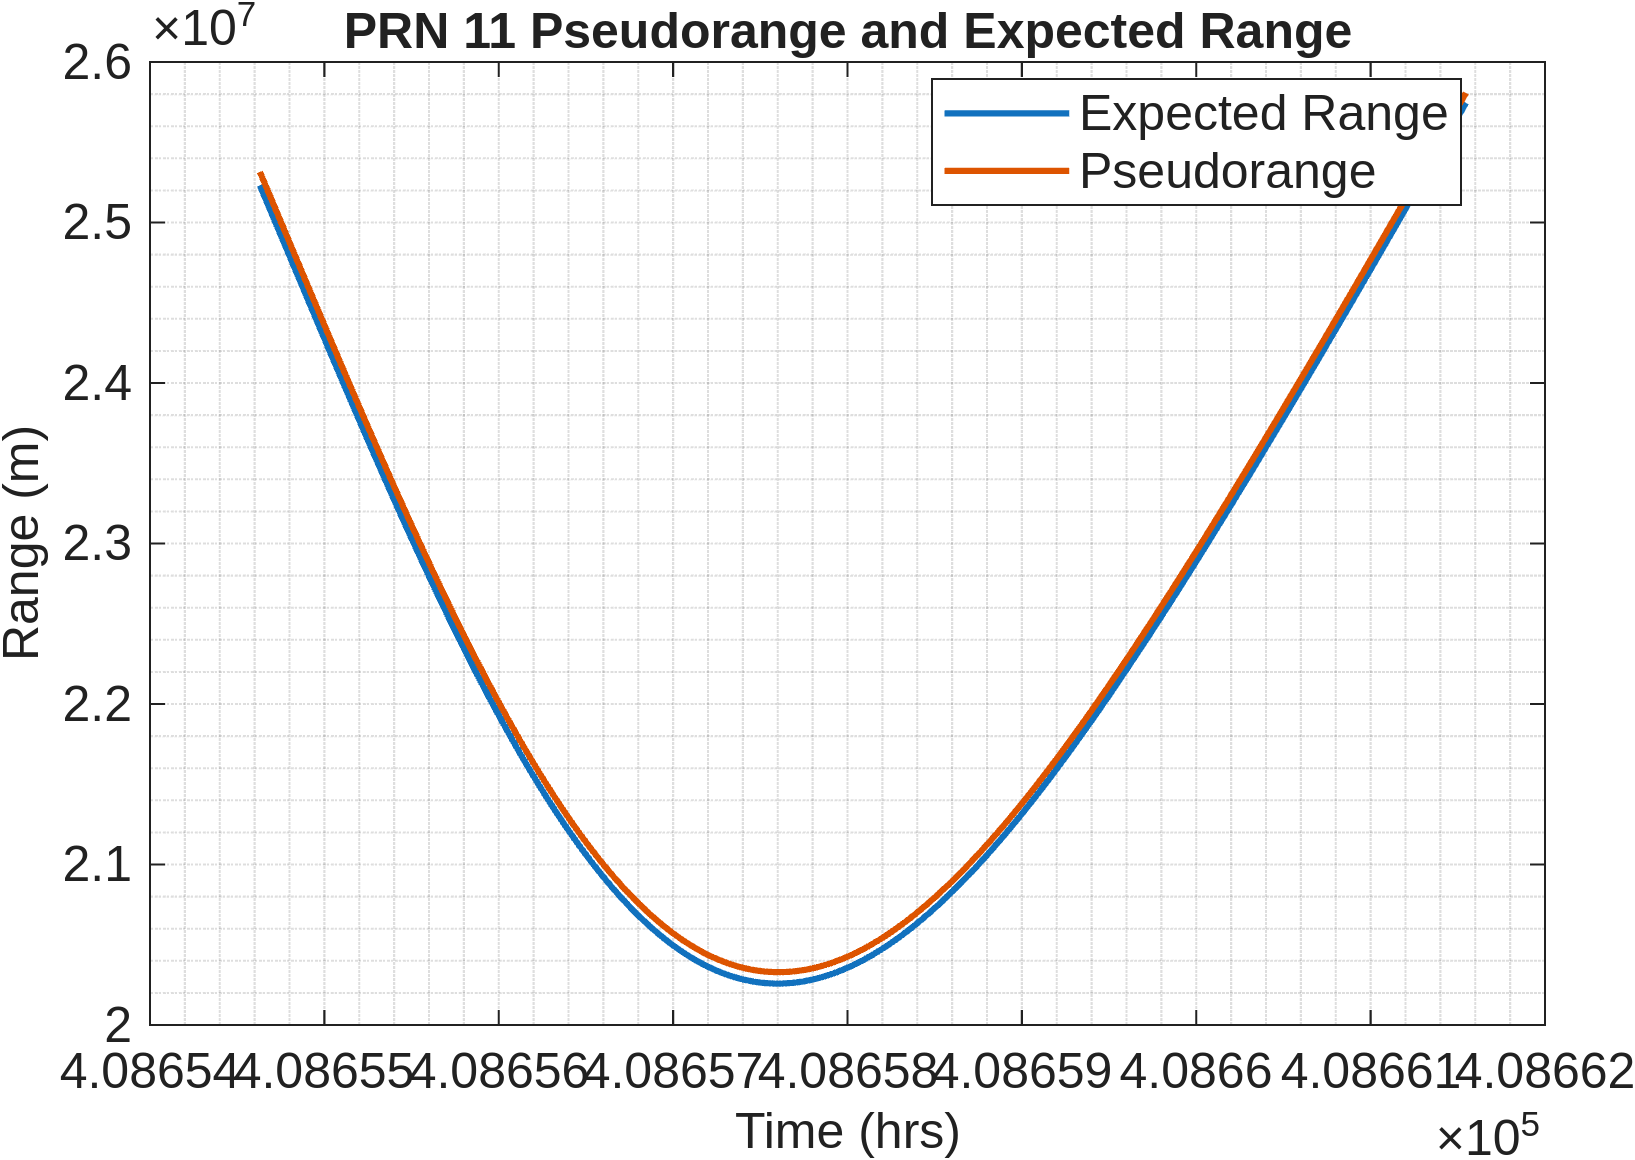
\includegraphics[width=0.6\textwidth]{../MATLAB/figures/HW3_P5_pseudorange_vs_expected_PRN11.png}
    \caption{PRN11 C1C Pseudorange vs Expected Range}
    \label{fig:PRN11 C1C Pseudorange vs Expected Range}
\end{figure}

\begin{figure}[H]
    \centering
    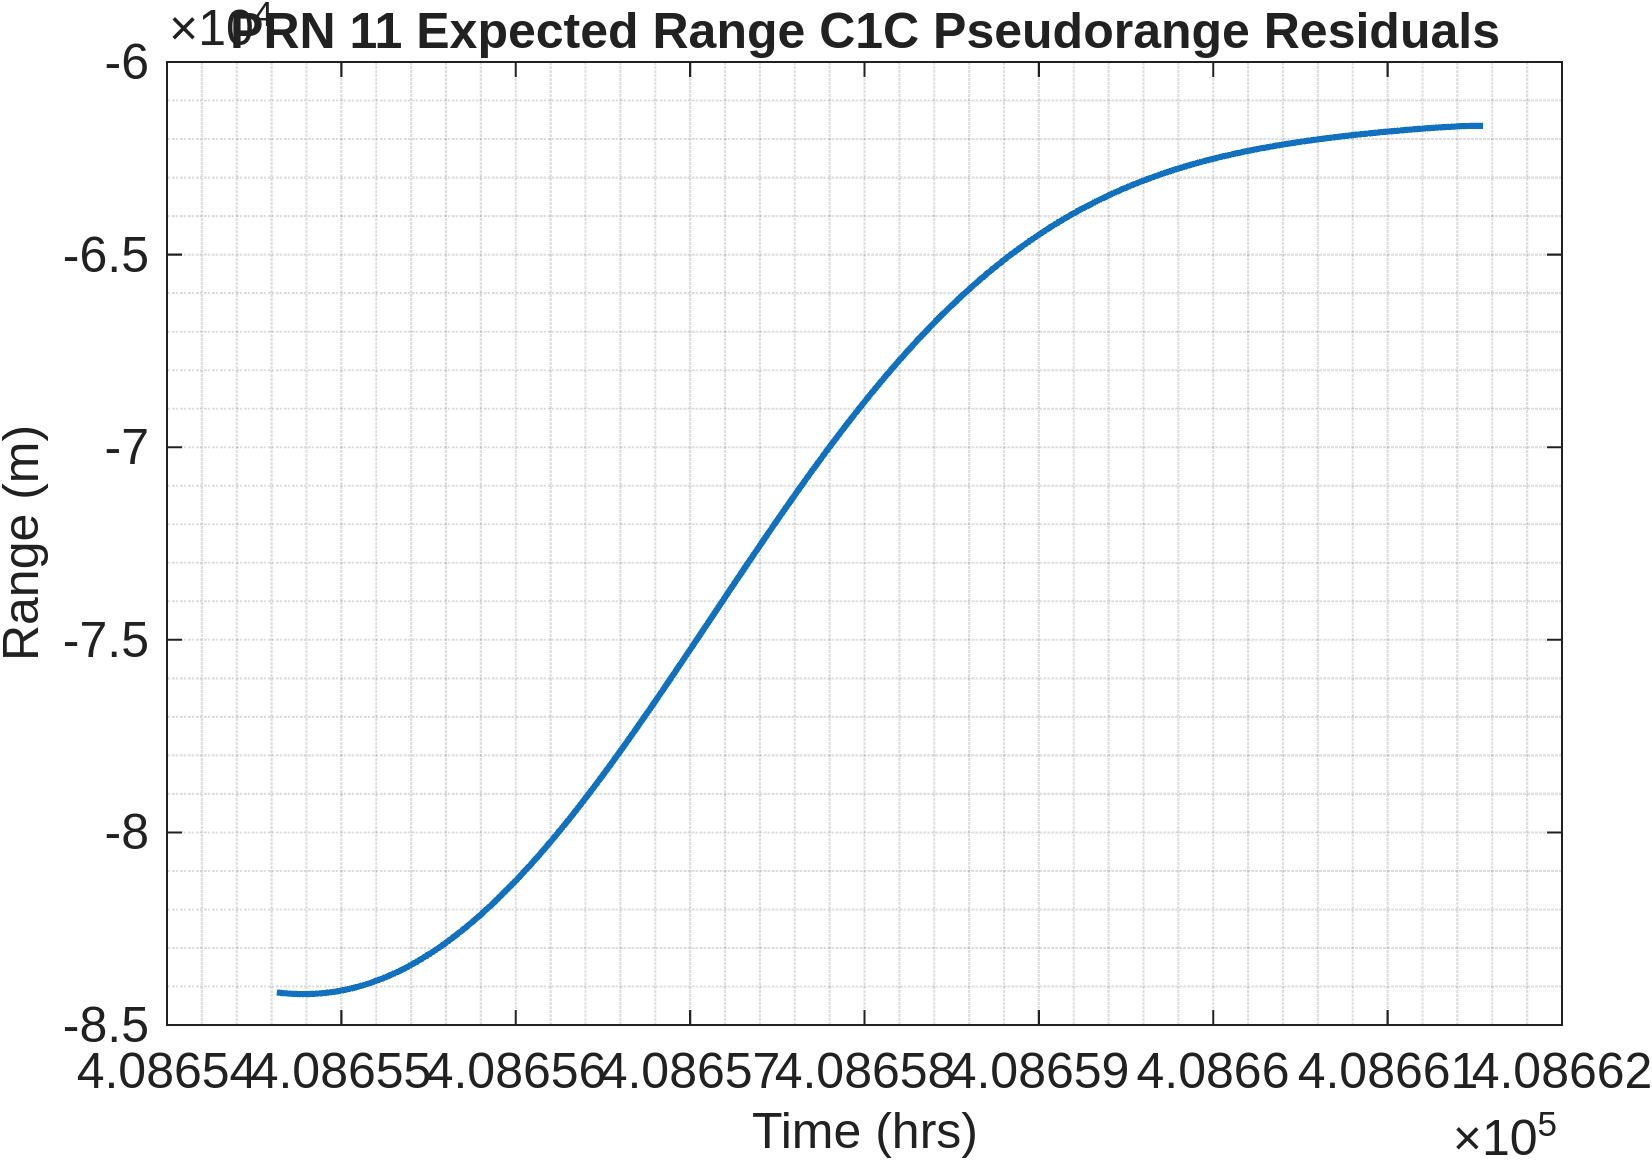
\includegraphics[width=0.6\textwidth]{../MATLAB/figures/HW3_P5_residuals_PRN11.png}
    \caption{PRN11 C1C Pseudorange vs Expected Range Residuals}
    \label{fig:PRN11 C1C Pseudorange vs Expected Range Residuals}
\end{figure}

\end{document}
